\chapter{Introduction}
As networks grow larger and more complex, redundancy becomes desirable and necessary.
With layer 2 (the data link layer in the OSI model, where we have MAC addresses but no IP addresses) redundancy also brings loops and the danger of so called Broadcast Storms (where broadcast messages are bounced back and forth between network nodes).
Because of this the Spannning Tree Protocol (STP)\cite{perlman85} was created.
The STP works by creating a logical overlay network (which has the form of a tree) over the physical network by disabling specific ports.
An example is shown in Figure~\ref{fig:stp_example}

\begin{figure}[h]
    \begin{center}
    \begin{subfigure}[b]{0.4\textwidth}
    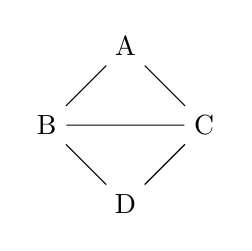
\begin{tikzpicture}
    \node (A) at (2,4) {A};
    \node (B) at (1,3) {B};
    \node (C) at (3,3) {C};
    \node (D) at (2,2) {D};

    \draw
    (A) -- (B)
    (A) -- (C)
    (B) -- (C)
    (B) -- (D)
    (C) -- (D);
    \end{tikzpicture}
    \caption{Physical topology}
    \end{subfigure}
    ~
    \begin{subfigure}[b]{0.4\textwidth}
    \begin{tikzpicture}
    \node (root) at (2,4) {A};
    \node (B) at (1,3) {B};
    \node (C) at (3,3) {C};
    \node (D) at (2,2) {D};

    \draw
    (root) -- (B)
    (root) -- (C)
    (B) -- (D);
    \end{tikzpicture}
    \caption{Logical topology}
    \end{subfigure}
    \end{center}
    \caption{An example of how STP changes the logical network topology}
    \label{fig:stp_example}
\end{figure}

Note that the only layer 2 hardware considered in this paper will be Switches, as Hubs are not STP capable and also very rarely used in larger networks.
We will also refer to Switches as Bridges, in order to be compliant with the STP nomenclature\\

As the networks STP is used in are complex to begin with, and as changes and outages are not immediately (if ever) noticed, it can be difficult to keep tabs on the current network layout.
Debugging STP configurations is also a difficult and time consuming task.
While possible, surveying the results of the STP algorithm via the Simple Network Management Protocol (SNMP) - which many business-grade Bridges are capable of - is tedious and requires the administrator to connect to every single Switch in the Local Area Network (LAN).
The aim of this project and the resulting STP-Tree-Generator (referred to in this simply paper as the Generator) is to decrease the complexity and workload that this task requires.\\

It achieves this goal by gathering information about the STP topology in a distributed fashion, and then using this information to generate a visualization of the network.
The visualization is generated by a central server by combining the data sent by multiple nodes.
A network administrator can then query said visualization from the server.
As of the time of writing this paper, the only output format available is in the form of \textit{.tikz} drawings to be used in \LaTeX.
